% !TeX spellcheck = en_GB
%%%%%%%%%%%%%%%%%%%%%%%%%%%%%%%%%%%%%%%%%%%%%%%%%%%%%%%%%%%%%%%%%%%%%%%%%%%%%%%%
%\documentclass[handout]{beamer}\mode<handout>{\usetheme{default}}
%
\documentclass[presentation]{beamer}\mode<presentation>{\usetheme{blackAMSBolognaFC}}
%\documentclass[handout]{beamer}\mode<handout>{\usetheme{AMSBolognaFC}}
% \setbeamertemplate{bibliography item}{\insertbiblabel}
%%%%%%%%%%%%%%%%%%%%%%%%%%%%%%%%%%%%%%%%%%%%%%%%%%%%%%%%%%%%%%%%%%%%%%%%%%%%%%%%
\usepackage[english]{babel}
\usepackage[utf8]{inputenc}
%
\usepackage{magnini-dc-kr-2023}
%%%%%%%%%%%%%%%%%%%%%%%%%%%%%%%%%%%%%%%%%%%%%%%%%%%%%%%%%%%%%%%%%%%%%%%%%%%%%%%%
\title[Symbolic Transfer Learning]{
    % same title of the presented paper
    \textbf{Symbolic Transfer Learning through}
    \\
    \textbf{Knowledge Manipulation Methods}
}
%
% \subtitle{Extended Abstract}
%
% same authors order of the presented paper
\author[Magnini]{
	\emph{Matteo Magnini}$^{*}$ % empth the presenting author
}
%
\institute[UniBo]{
    $^{*}$Dipartimento di Informatica -- Scienza e Ingegneria (DISI)
    \\
    \textsc{Alma Mater Studiorum} -- Università di Bologna
    \\
    \texttt{
        \emph{matteo.magnini}@unibo.it % emph the presenting author's email
    }
}
%
\date[DC KR 2023]{
	Doctoral Consortium at the
    \\
    20\textsuperscript{th} International Conference on
	\\
	Principles of Knowledge Representation and Reasoning (KR)
	\\
	September 5\textsuperscript{th}, 2023, Rhodes (Greece)
}
%%%%%%%%%%%%%%%%%%%%%%%%%%%%%%%%%%%%%%%%%%%%%%%%%%%%%%%%%%%%%%%%%%%%%%%%%%%%%%%%
\AtBeginSection[]
{
%\\\\\\\\\\\\\\\\\\\\\
\begin{frame}<beamer>[c,noframenumbering]
\frametitle{Next in Line\ldots}
\tableofcontents[sectionstyle=show/shaded,subsectionstyle=hide]
\end{frame}
%\\\\\\\\\\\\\\\\\\\\\
}
\AtBeginSubsection[]
{
%\\\\\\\\\\\\\\\\\\\\\
\begin{frame}<beamer>[shrink,noframenumbering]
    \frametitle{Focus on\ldots}
	\mbox{~}
	\tableofcontents[currentsubsection,sectionstyle=shaded,subsectionstyle=show/shaded]
	\mbox{~}
\end{frame}
%\\\\\\\\\\\\\\\\\\\\\
}
%%%%%%%%%%%%%%%%%%%%%%%%%%%%%%%%%%%%%%%%%%%%%%%%%%%%%%%%%%%%%%%%%%%%%%%%%%%%%%%%
\begin{document}
%%%%%%%%%%%%%%%%%%%%%%%%%%%%%%%%%%%%%%%%%%%%%%%%%%%%%%%%%%%%%%%%%%%%%%%%%%%%%%%%

%\\\\\\\\\\\\\\\\\\\\\
\frame{\titlepage}
%\\\\\\\\\\\\\\\\\\\\\

%===============================================================================
\section{Motivation \& Context}
%===============================================================================

%\\\\\\\\\\\\\\\\\\\\\
\begin{frame}[c]{Context}

    Players involved in a Machine Learning workflow:
    \vspace{0.5cm}
    \begin{itemize}
        \item Data
        %
        \begin{itemize}
            \item[!] require \alert{labels}
        \end{itemize}

        \vfill

        \item Knowledge
        %
        \begin{itemize}
            \item human experts
            \item common sense
            \item extracted from data/models
        \end{itemize}

        \vfill

        \item Model
        %
        \begin{itemize}
            \item trained on data
            \item sometimes also trained with prior knowledge
        \end{itemize}

    \end{itemize}
\end{frame}
%\\\\\\\\\\\\\\\\\\\\\

%\\\\\\\\\\\\\\\\\\\\\
\begin{frame}[allowframebreaks]{Utopy and Reality}

    \hspace{0.5cm}
    \includegraphics[width=0.4\textwidth]{figures/data-labels-knowledge-1}
    \hfill

    \framebreak

    \hfill
    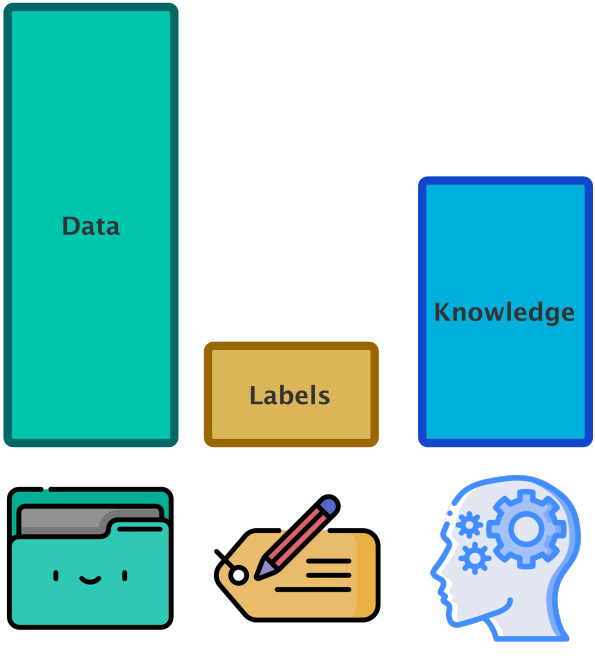
\includegraphics[width=0.4\textwidth]{figures/data-labels-knowledge-2}
    \hspace{0.5cm}

    \framebreak

    \centering
    But in some tasks we deal with both low data/labels and knowledge\dots

\end{frame}
%\\\\\\\\\\\\\\\\\\\\\

%\\\\\\\\\\\\\\\\\\\\\
\begin{frame}[allowframebreaks]{Transfer Learning}

    \centering
    Reuse the knowledge acquired in a \alert{similar} task!

    \framebreak

    \begin{figure}
        \includegraphics[width=0.7\textwidth]{figures/transfer-learning}
    \end{figure}

    \framebreak


\end{frame}
%\\\\\\\\\\\\\\\\\\\\\

%===============================================================================
\section{Symbolic Transfer Learning Framework}
%===============================================================================

%\\\\\\\\\\\\\\\\\\\\\
\begin{frame}%[allowframebreaks]
\frametitle{Theory / modelling / design}

    Provide 2-3 slides discussing the Theory / modelling / design

\end{frame}
%\\\\\\\\\\\\\\\\\\\\\

%===============================================================================
\section{Where we are now}
%===============================================================================

%\\\\\\\\\\\\\\\\\\\\\
\begin{frame}%[allowframebreaks]
\frametitle{Case study / Experiments / Results}

    Provide 2-3 slides discussing the Case study / Experiments / Results of the paper

\end{frame}
%\\\\\\\\\\\\\\\\\\\\\

\section{Where we are going}

%\\\\\\\\\\\\\\\\\\\\\
\begin{frame}%[allowframebreaks]
\frametitle{Conclusions \& future works}

\begin{block}{Summing up}
    Summarise the most relevant contributions of this study:
    %
    \begin{itemize}
        \item conclusion 1
        \item conclusion 2
        \item conclusion 3
    \end{itemize}
\end{block}

\begin{exampleblock}{Future works}
    Sketch some future research directions
    %
    \begin{itemize}
        \item future work 1
        \item future work 2
    \end{itemize}
\end{exampleblock}

(may be split into 2 slides)

\end{frame}
%\\\\\\\\\\\\\\\\\\\\\

%===============================================================================
\section*{}
%===============================================================================
\frame{\titlepage}

%===============================================================================
\section*{\bibname}
%===============================================================================

\setbeamertemplate{page number in head/foot}{}
%\\\\\\\\\\\\\\\\\\\\\

\begin{frame}[t,allowframebreaks,noframenumbering]\frametitle{\refname}
% \begin{frame}[c]\frametitle{\refname}
	\footnotesize
%	\scriptsize
    \bibliographystyle{apalike-AMS}
    % \bibliographystyle{plain}
    % \nocite{*}
	\bibliography{magnini-dc-kr-2023}
\end{frame}
%\\\\\\\\\\\\\\\\\\\\\

%%%%%%%%%%%%%%%%%%%%%%%%%%%%%%%%%%%%%%%%%%%%%%%%%%%%%%%%%%%%%%%%%%%%%%%%%%%%%%%%
\end{document}
%%%%%%%%%%%%%%%%%%%%%%%%%%%%%%%%%%%%%%%%%%%%%%%%%%%%%%%%%%%%%%%%%%%%%%%%%%%%%%%%
